\documentclass[12pt, titlepage]{article}
\usepackage{graphicx}
\usepackage{float}
\restylefloat{table}

% Imported Packages
%------------------------------------------------------------------------------
\usepackage{amssymb}
\usepackage{amstext}
\usepackage{amsthm}
\usepackage{amsmath}
\usepackage{enumerate}
\usepackage{fancyhdr}
\usepackage[margin=1in]{geometry}
\usepackage{graphicx}
\usepackage{extarrows}
\usepackage{setspace}
%------------------------------------------------------------------------------

% Header and Footer
%------------------------------------------------------------------------------
\pagestyle{plain}  
\renewcommand\headrulewidth{0.4pt}                                      
\renewcommand\footrulewidth{0.4pt}                    

\newcommand\tab[1][1cm]{\hspace*{#1}}                
%------------------------------------------------------------------------------

% Title Details
%------------------------------------------------------------------------------
\title{SE 3A04: Software Design III: Large System Design}
\author{Group \#5, Spaceship System Sabotage %Alliteration; always adored and absolutely amazing
		\\Pareek Ravi 001407109
		\\Pavle Arezina 001410366
		\\David Hobson 001412317
		\\Victoria Graff 001401451
		\\Julian Cassano 001406891
}
\date{\today}                               
%------------------------------------------------------------------------------

% Document
%------------------------------------------------------------------------------
\begin{document}
\maketitle	
\pagenumbering{arabic}
\tableofcontents
\listoftables
\listoffigures
\newpage

\section{Introduction}
\label{sec:introduction}
% Begin Section


\subsection{Purpose}
\label{sub:purpose}
% Begin SubSection
\tab The Large System Design document is responsible for the high level architecture design of the system and the results produced from this analysis will be utilized in the design phase. The document is derived from the requirements and specifications of the overall system, determined in the previous software requirement specification document. The intended audience of the document is mainly for the developers who will be utilizing the large system design document to understand the overall design of the program to help structure the responsibilities assigned to each class. Developers who are maintaining the program may also use the document to ensure new additions to the program follow the system design properly to ensure a smooth experience for the user.
% End SubSection

\subsection{System Description}
\label{sub:system_description}
\tab Space system sabotage is a simulation of a fictional spaceship that is travelling to a pre-determined location in a fixed amount of time. The user will interact with the system through random events based on a function of the running time of the simulation. Random events will involve negative situations that occur, such as comets damaging the ship or part of the ship being sabotaged, where the user will have to respond to fix them in a timely manner with a selection of tools. If successful, the space ship continues toward its goal but if an incorrect solution was chosen then the problem is spread to other systems. If enough events happen with incorrect solutions to them, then the space ship will slowly spiral out of control and the user will fail the simulation. This system offers an entertaining environment to the user where they will be challenged to keep the spaceship intact until it dock import at the space station.
% End SubSection

\subsection{Overview}
\label{sub:overview}
\tab The rest of the Large System Design document is separated into four sections, the first being the use case diagram. This diagram models the functionality of the system using actors, the users of the system, and use cases of the system. The next section is the analysis class diagram which describes the key classes of a system and their interrelationship through boundary class, entity classes, and controller classes. These classes of the system are identified by extracting through the description of the use case descriptions.  Section three should provide an overview of the overall architectural design of the application where the division of the system into subsystems follows high cohesion and low coupling. Last section is the Class Responsibility Collaborator (CRC) cards on the classes in the analysis class diagram where each card identifies and assigns responsibilities to classes required to build the system. After these four sections there is an appendix that includes the division of labour.
% End SubSection

% End Section
\newpage
\section{Use Case Diagram}
\label{sec:use_case_diagram}
% Begin Section
\begin{figure}[ht!]
\centering
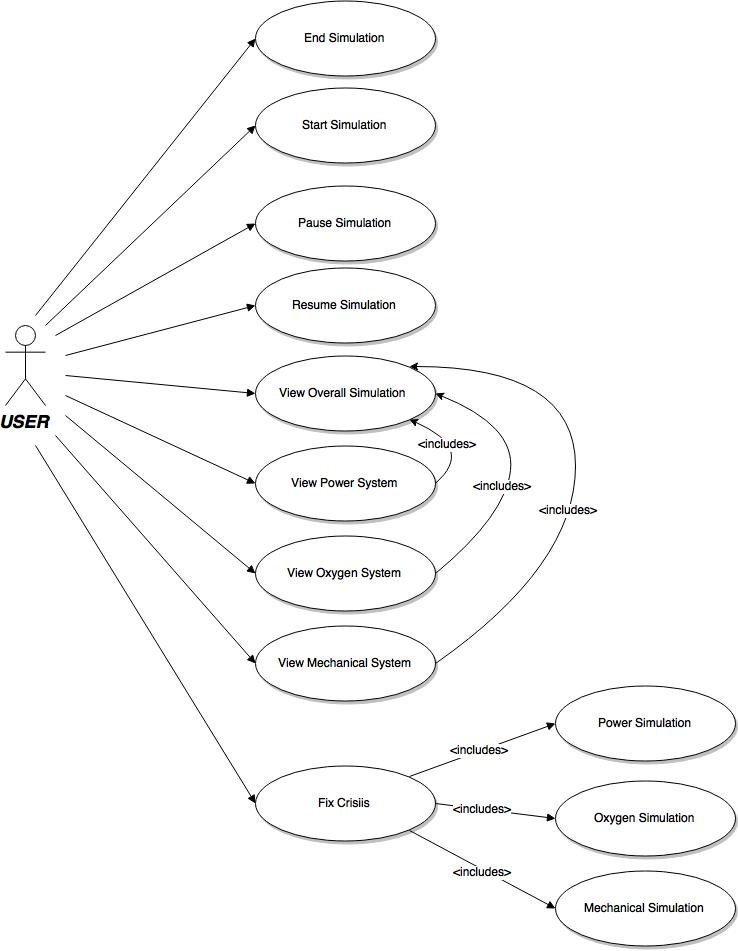
\includegraphics[width=120mm]{UseCase.jpg}
\caption{Use Case Diagram \label{usecase}}
\end{figure}
\subsection*{Use Case Definitions}
\begin{enumerate}[a)]
	\item End Simulation: The user is in a play session and intends to indefinitely stop the simulation and return to the main menu.
	\item Start Simulation: The user is in the main menu and intends to begin a play session.
	\item Pause Simulation: The user is in a play session and intends to pause the simulation but intends to resume at a later time.
	\item Resume Simulation: The user is in a paused play session and intends to resume and continue the simulation.
	\item View Overall System: The user is in a play session and intends to display the status of all the subsystems at once.
	\item View Power System: The user is in a play session and intends to include the status of the Power System in the displayed view.
	\item View Oxygen System: The user is in a play session and intends to include the status of the Oxygen System in the displayed view.
	\item View Mechanical System: The user is in a play session and intends to include the status of the Mechanical System in the displayed view.
	\item Fix Crisis: The user is in a play session and intends to resolve an event that is negatively affecting one of the subsystems.
	\item Fix Power: The user is in a fix crisis event and intends to resolve an event affecting the power system.
	\item Fix Oxygen: The user is in a fix crisis event and intends to resolve an event affecting the oxygen system.
	\item Fix Mechanical: The user is in a fix crisis event and intends to resolve an event affecting the mechanical system.
\end{enumerate}
% End Section
\newpage
\section{Analysis Class Diagram}
\label{sec:analysis_class_diagram}
% Begin Section
\begin{figure}[ht!]
\centering
\includegraphics[width=120mm]{"Analysis Class Diagram".jpg}
\caption{Analysis Class Diagram of System \label{analysisclass}}
\end{figure}
% End Section


\section{Architectural Design}
\label{sec:architectural_design}
% Begin Section
This section should provide an overview of the overall architectural design of your application. You overall architecture should show the division of the system into subsystems with high cohesion and low coupling.

\subsection{System Architecture}
\label{sub:system_architecture}
% Begin SubSection
The main controller of the system is the primary interaction point for all classes. Every time a use case event is instantiated, the main controller will be prompted to interact with the specific class that is associated with the attempted performed action. This means that each class that can return values will be dependent on the main controller in order to receive a prompt at the correct time. The system is a presentation-abstraction-control (PAC) architecture, being similar to MVC but not identical. The reason this architecture style was chosen is because we wanted each section of the architecture to only interact through the controller, to reduce conflict and clutter in the classes. The following diagram shows the main controller interacting with each set of classes individually, with no interaction directly between classes.

\begin{figure}[h!]
  \centering
  \includegraphics[scale=0.5]{"Overall Architecture".jpg}
  \caption{Structural architecture diagram for the PAC system.}
\end{figure}
% End SubSection

\subsection{Subsystems}
\label{sub:subsystems}
% Begin SubSection
\begin{itemize}
\item The power subsystem controls all of the all of the interactions that relate to the simulated amount of electrical power in the system and is dependent on the main controller. This subsystem can "malfunction" and must be stimulated to return to base state.
\item The oxygen subsystem controls all of the interactions that relate to the simulated amount of air in the system and is dependent on the main controller. This subsystem can "malfunction" and must be stimulated to return to base state.
\item The mechanical subsystem controls all of the interactions that relate to the simulated physical moving parts in the system and is dependent on the main controller. This subsystem can "malfunction" and must be stimulated to return to base state.
\item The tool subsystem controls all of the interactions that will "fix" the other simulated subsystems and return them to normal state.
\item The menu subsystem controls all interactions outside of the play session and will allow the user to performa actions such as pausing, resuming, or quitting the play session.
\item The main controller subsystem is the main hub of interaction between all other subsystems and will apporpriately stimulate each subsystem at the correct time. This subsystem receives input from all other subsystems and returns the output back to each system to determine what will happen in the simulation.
\end{itemize}
% End SubSection

% End Section
	
\section{Class Responsibility Collaboration (CRC) Cards}
\label{sec:class_responsibility_collaboration_crc_cards}
% Begin Section
This section should contain all of your CRC cards.

\begin{enumerate}[a)]
	\item Provide a CRC Card for each identified class
	\item Please use the format outlined in tutorial, i.e., 
	\begin{table}[ht]
		\centering
		\begin{tabular}{|p{5cm}|p{5cm}|}
		\hline 
		 \multicolumn{2}{|l|}{\textbf{Class Name:}} \\
		\hline
		\textbf{Responsibility:} & \textbf{Collaborators:} \\
		\hline
		\vspace{1in} & \\
		\hline
		\end{tabular}
	\end{table}

%Start Screen	
	\begin{table}[H]
		\centering
		\begin{tabular}{|p{5cm}|p{5cm}|}
		\hline 
		 \multicolumn{2}{|l|}{\textbf{Class Name: Start Screen}} \\
		\hline
		\textbf{Responsibility:} & \textbf{Collaborators:} \\
		\hline
		 Receive request to display a prompt to start game& Menu Controller \\
		\hline
		 Display screen message to user& \\
		\hline
		 Respond to prompt being pressed by user& \\
		\hline
		 Send request to Menu Controller to start game& Menu Controller \\
		\hline
		\end{tabular}
	\end{table}
	
%End Screen	
	\begin{table}[H]
		\centering
		\begin{tabular}{|p{5cm}|p{5cm}|}
		\hline 
		 \multicolumn{2}{|l|}{\textbf{Class Name: End Screen}} \\
		\hline
		\textbf{Responsibility:} & \textbf{Collaborators:} \\
		\hline
		 Receive request to display a prompt to end game& Menu Controller \\
		\hline
		 Display screen message to user& \\
		\hline
		 Respond to prompt being pressed by user& \\
		\hline
		 Send request to Menu Controller to end game& Menu Controller \\
		\hline
		\end{tabular}
	\end{table}
	
%Pause Screen	
	\begin{table}[H]
		\centering
		\begin{tabular}{|p{5cm}|p{5cm}|}
		\hline 
		 \multicolumn{2}{|l|}{\textbf{Class Name: Pause Screen}} \\
		\hline
		\textbf{Responsibility:} & \textbf{Collaborators:} \\
		\hline
		 Receive request to display a prompt to pause game& Menu Controller \\
		\hline
		 Display screen message to user& \\
		\hline
		 Respond to prompt being pressed by user& \\
		\hline
		 Send request to Menu Controller to pause and unpause game& Menu Controller \\
		\hline
		\end{tabular}
	\end{table}
	
%Success Screen	
	\begin{table}[H]
		\centering
		\begin{tabular}{|p{5cm}|p{5cm}|}
		\hline 
		 \multicolumn{2}{|l|}{\textbf{Class Name: Success Screen}} \\
		\hline
		\textbf{Responsibility:} & \textbf{Collaborators:} \\
		\hline
		 Receive request to display a screen message when game has been won& Menu Controller \\
		\hline
		 Display screen message to user& \\
		\hline
		\end{tabular}
	\end{table}
	
%Failure Screen	
	\begin{table}[H]
		\centering
		\begin{tabular}{|p{5cm}|p{5cm}|}
		\hline 
		 \multicolumn{2}{|l|}{\textbf{Class Name: Failure Screen}} \\
		\hline
		\textbf{Responsibility:} & \textbf{Collaborators:} \\
		\hline
		 Receive request to display a screen message when game has been lost& Menu Controller \\
		\hline
		 Display screen message to user& \\
		\hline
		\end{tabular}
	\end{table}	

%Choose Tool
	\begin{table}[H]
		\centering
		\begin{tabular}{|p{5cm}|p{5cm}|}
		\hline 
		 \multicolumn{2}{|l|}{\textbf{Class Name: Choose Tool}} \\
		\hline
		\textbf{Responsibility:} & \textbf{Collaborators:} \\
		\hline
		 A view for the user the select the tool they wish to use to fix the issue on the spaceship & Tool Controller\\
		\hline
		\end{tabular}
	\end{table}
	
%Tool Fail
	\begin{table}[H]
		\centering
		\begin{tabular}{|p{5cm}|p{5cm}|}
		\hline 
		 \multicolumn{2}{|l|}{\textbf{Class Name: Tool Fail}} \\
		\hline
		\textbf{Responsibility:} & \textbf{Collaborators:} \\
		\hline
		 A view to show the user that they chose the wrong tool to fix the issue & Tool Controller\\
		\hline
		\end{tabular}
	\end{table}

%Tool Success
	\begin{table}[H]
		\centering
		\begin{tabular}{|p{5cm}|p{5cm}|}
		\hline 
		 \multicolumn{2}{|l|}{\textbf{Class Name: Tool Success}} \\
		\hline
		\textbf{Responsibility:} & \textbf{Collaborators:} \\
		\hline
		 A view to show the user that they chose the correct tool to fix the issue & Tool Controller\\
		\hline
		\end{tabular}
	\end{table}

%Event Alert
	\begin{table}[H]
		\centering
		\begin{tabular}{|p{5cm}|p{5cm}|}
		\hline 
		 \multicolumn{2}{|l|}{\textbf{Class Name: Event Alert}} \\
		\hline
		\textbf{Responsibility:} & \textbf{Collaborators:} \\
		\hline
		 A view to show the user that there is an issue with the spaceship & Tool Controller\\
		\hline
		\end{tabular}
	\end{table}

%Event Timer
	\begin{table}[H]
		\centering
		\begin{tabular}{|p{5cm}|p{5cm}|}
		\hline 
		 \multicolumn{2}{|l|}{\textbf{Class Name: Event Timer}} \\
		\hline
		\textbf{Responsibility:} & \textbf{Collaborators:} \\
		\hline
		 A timer to handle the duration of an event & Tool Controller\\
		\hline
		\end{tabular}
	\end{table}

%Tool Controller
	\begin{table}[H]
		\centering
		\begin{tabular}{|p{5cm}|p{5cm}|}
		\hline 
		 \multicolumn{2}{|l|}{\textbf{Class Name: Tool Controller}} \\
		\hline
		\textbf{Responsibility:} & \textbf{Collaborators:} \\
		\hline
		 Get user's tool choice & Choose Tool\\
		\hline
		 Determine if it was the correct tool to use & Tool Success, Tool Fail \\
		\hline
		 Inform the user of an issue & Event Alert \\
		\hline
		 Know the event has occured & Overall Controller \\
		\hline
		\end{tabular}
	\end{table}

%Power Model
	\begin{table}[H]
		\centering
		\begin{tabular}{|p{5cm}|p{5cm}|}
		\hline 
		 \multicolumn{2}{|l|}{\textbf{Class Name: Power Model}} \\
		\hline
		\textbf{Responsibility:} & \textbf{Collaborators:} \\
		\hline
		 Hold the information of the power system & \\
		\hline
		\end{tabular}
	\end{table}

%Power View
	\begin{table}[H]
		\centering
		\begin{tabular}{|p{5cm}|p{5cm}|}
		\hline 
		 \multicolumn{2}{|l|}{\textbf{Class Name: Power View}} \\
		\hline
		\textbf{Responsibility:} & \textbf{Collaborators:} \\
		\hline
		 DIsplay the power system to the user & Power Controller\\
		\hline
		\end{tabular}
	\end{table}

%Power Controller
	\begin{table}[H]
		\centering
		\begin{tabular}{|p{5cm}|p{5cm}|}
		\hline 
		 \multicolumn{2}{|l|}{\textbf{Class Name: Power Controller}} \\
		\hline
		\textbf{Responsibility:} & \textbf{Collaborators:} \\
		\hline
		Updates subsystem information after tool usage & Power Model, Overall Controller\\
		\hline
		 Tells system of subsystem information & Power Model, Overall Controller\\
		\hline
		 Indicate to the view what to display & Power View, Power Model\\
		\hline
		 Generate the stimulation based on a time & Overall Controller \\
		\hline
		\end{tabular}
	\end{table}

%Oxygen Model
	\begin{table}[H]
		\centering
		\begin{tabular}{|p{5cm}|p{5cm}|}
		\hline 
		 \multicolumn{2}{|l|}{\textbf{Class Name: Oxygen Model}} \\
		\hline
		\textbf{Responsibility:} & \textbf{Collaborators:} \\
		\hline
		 Hold the information of the oxygen system & \\
		\hline
		\end{tabular}
	\end{table}

%Oxygen View
	\begin{table}[H]
		\centering
		\begin{tabular}{|p{5cm}|p{5cm}|}
		\hline 
		 \multicolumn{2}{|l|}{\textbf{Class Name: Oxygen View}} \\
		\hline
		\textbf{Responsibility:} & \textbf{Collaborators:} \\
		\hline
		 DIsplay the oxygen system to the user & Oxygen Controller\\
		\hline
		\end{tabular}
	\end{table}

%Oxygen Controller
	\begin{table}[H]
		\centering
		\begin{tabular}{|p{5cm}|p{5cm}|}
		\hline 
		 \multicolumn{2}{|l|}{\textbf{Class Name: Oxygen Controller}} \\
		\hline
		\textbf{Responsibility:} & \textbf{Collaborators:} \\
		\hline
		Updates subsystem information after tool usage & Oxygen Model, Overall Controller\\
		\hline
		 Tells system of subsystem information & Oxygen Model, Overall Controller\\
		\hline
		 Indicate to the view what to display & Oxygen Model, Oxygen View\\
		\hline
		 Generate the stimulation based on a time & Overall Controller \\
		\hline
		\end{tabular}
	\end{table}

%Mechanical Model
	\begin{table}[H]
		\centering
		\begin{tabular}{|p{5cm}|p{5cm}|}
		\hline 
		 \multicolumn{2}{|l|}{\textbf{Class Name: Mechanical Model}} \\
		\hline
		\textbf{Responsibility:} & \textbf{Collaborators:} \\
		\hline
		 Hold the information of the mechanical system & \\
		\hline
		\end{tabular}
	\end{table}

%Mechanical View
	\begin{table}[H]
		\centering
		\begin{tabular}{|p{5cm}|p{5cm}|}
		\hline 
		 \multicolumn{2}{|l|}{\textbf{Class Name: Mechanical View}} \\
		\hline
		\textbf{Responsibility:} & \textbf{Collaborators:} \\
		\hline
		 DIsplay the mechanical system to the user & Mechanical Controller\\
		\hline
		\end{tabular}
	\end{table}

%Mechanical Controller
	\begin{table}[H]
		\centering
		\begin{tabular}{|p{5cm}|p{5cm}|}
		\hline 
		 \multicolumn{2}{|l|}{\textbf{Class Name: Mechanical Controller}} \\
		\hline
		\textbf{Responsibility:} & \textbf{Collaborators:} \\
		\hline
		Updates subsystem information after tool usage & Mechanical Model, Overall Controller\\
		\hline
		 Tells system of subsystem information & Mechanical Model, Overall Controller\\
		\hline
		 Indicate to the view what to display & Mechanical Model, Mechanical View\\
		\hline
		 Generate the stimulation based on a time & Overall Controller \\
		\hline
		\end{tabular}
	\end{table}

\end{enumerate}
% End Section

\appendix
\section{Division of Labour}
\label{sec:division_of_labour}
% Begin Section
Include a Division of Labour sheet which indicates the contributions of each team member. This sheet must be signed by all team members.
% End Section
\begin{table}[h!]
\centering

\begin{tabular}{|c|c|c|}
\hline
{\bf Member} & {\bf Duties}&{\bf Signature}\\
\hline
{David Hobson} & { } & { }\\
{} & {}  & {}\\
\hline
{Pavle Arezina} & {} & {}\\
{} & {} & {}\\
\hline
{Pareek Ravi} & {} & {}\\
{} & {} & {}\\
\hline
{Victoria Graff} & {} & {}\\
{} & {} & {}\\
\hline
{Julian Cassano} & {} & {}\\
{} & {} & {}\\
\hline
\end{tabular}

\end{table}

\newpage
\section*{IMPORTANT NOTES}
\begin{itemize}
%	\item You do \underline{NOT} need to provide a text explanation of each diagram; the diagram should speak for itself
	\item Please document any non-standard notations that you may have used
	\begin{itemize}
		\item \emph{Rule of Thumb}: if you feel there is any doubt surrounding the meaning of your notations, document them
	\end{itemize}
	\item Some diagrams may be difficult to fit into one page
	\begin{itemize}
		\item It is OK if the text is small but please ensure that it is readable when printed
		\item If you need to break a diagram onto multiple pages, please adopt a system of doing so and thoroughly explain how it can be reconnected from one page to the next; if you are unsure about this, please ask about it
	\end{itemize}
	\item Please submit the latest version of Deliverable 1 with Deliverable 2
	\begin{itemize}
		\item It does not have to be a freshly printed version; the latest marked version is OK
	\end{itemize}
	\item If you do \underline{NOT} have a Division of Labour sheet, your deliverable will \underline{NOT} be marked
\end{itemize}


\end{document}
%------------------------------------------------------------------------------